\documentclass[10pt]{mypackage}

% sans serif font:
%\usepackage{cmbright}
%\usepackage{sfmath}
%\usepackage{bbold} %better blackboard bold

%serif font + different blackboard bold for serif font
\usepackage{newpxtext,eulerpx}
\renewcommand*{\mathbb}[1]{\varmathbb{#1}}
\renewcommand*{\hbar}{\hslash}

\pagestyle{fancy} %better headers
\fancyhf{}
\rhead{Avinash Iyer}
\lhead{Ordinary Differential Equations: Homework 9}

\setcounter{secnumdepth}{0}

\begin{document}
\RaggedRight
\section{Part 1}%
\subsection{3.3, Problem 3}%
Finding the eigenvalues of the matrix, we have
\begin{align*}
  \det \begin{pmatrix}-5-\lambda & -2 \\ -1 & -4-\lambda\end{pmatrix} &= \left(5+\lambda\right)\left(4 + \lambda\right) -2\\
  \lambda^2 + 9\lambda +18 &= 0\\
  \left(\lambda + 6\right)\left(\lambda + 3\right) &= 0,
\end{align*}
so the eigenvalues are $\lambda_1 = -6$ and $\lambda_2 = -3$. Their corresponding eigenvectors are
\begin{align*}
  \vec{v}_1 &= \begin{pmatrix}2\\1\end{pmatrix}\\
  \vec{v}_2 &= \begin{pmatrix}-1\\1\end{pmatrix}.
\end{align*}
The phase portrait is as follows.
\begin{center}
  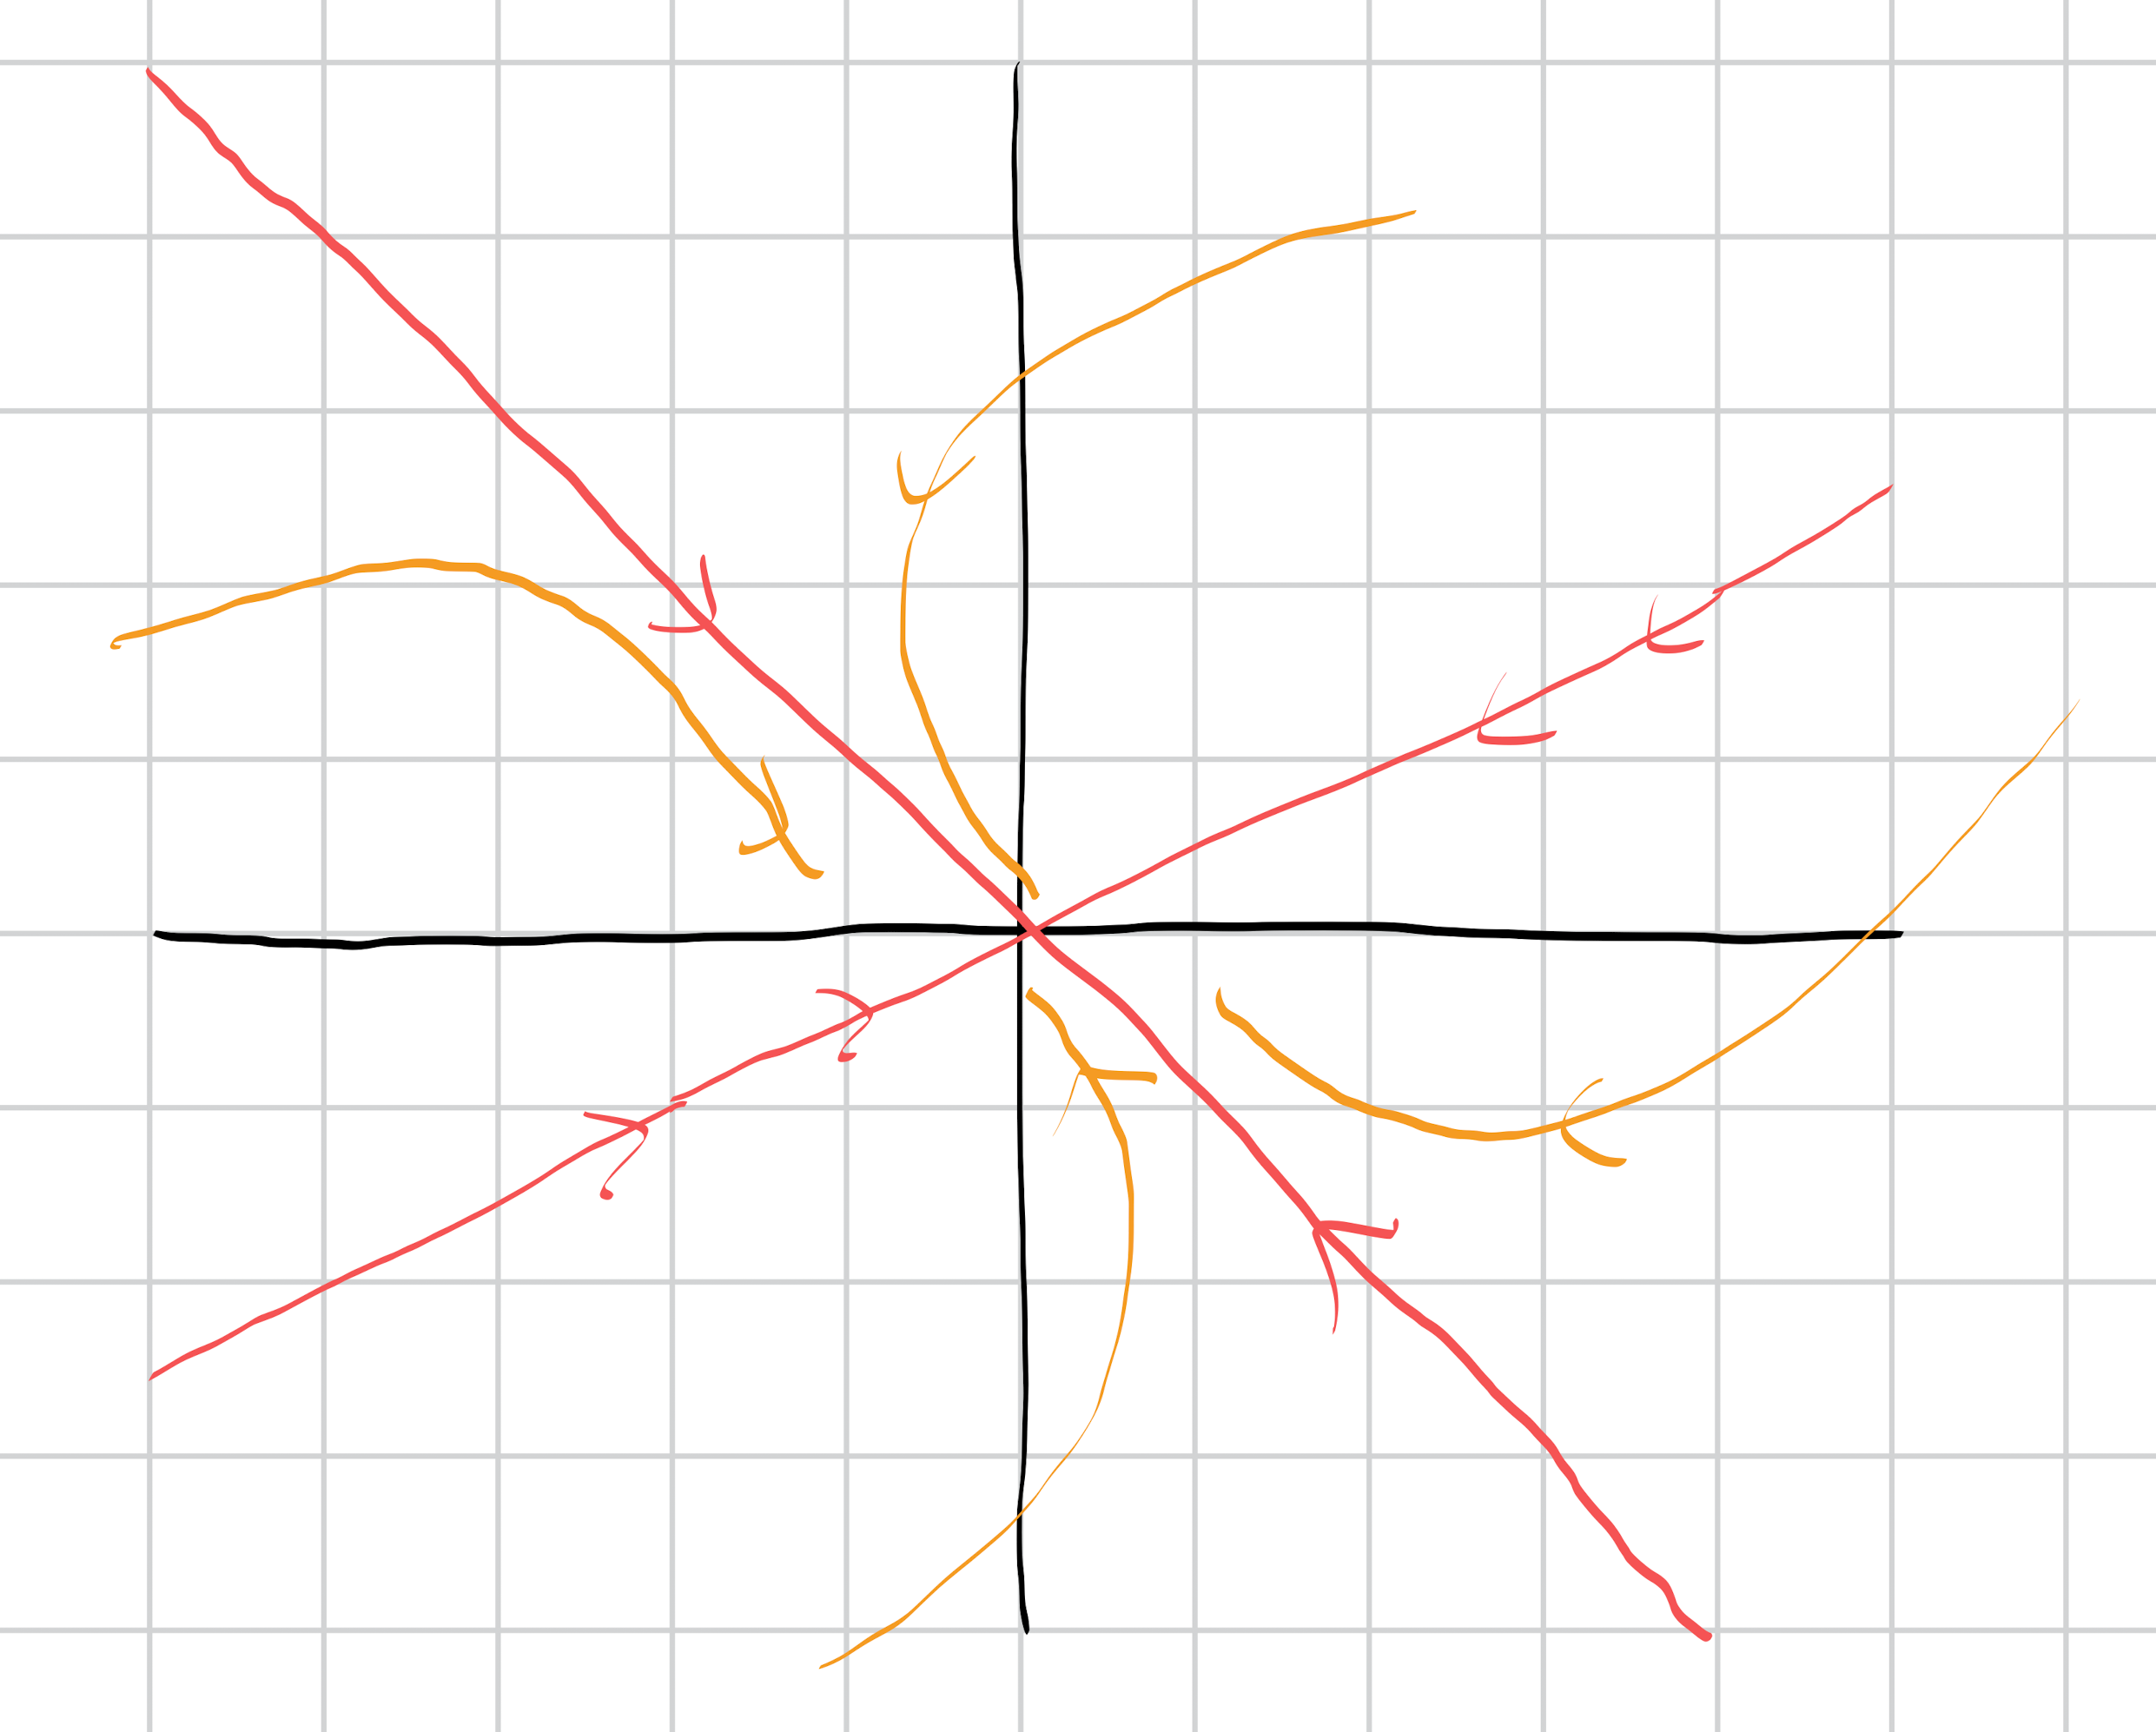
\includegraphics[width=7cm]{images/3_3_3.png}
\end{center}
\subsection{3.3, Problem 4}%
Finding the eigenvalues of the matrix, we have
\begin{align*}
  \det \begin{pmatrix}5-\lambda & 4 \\ 9 & 0-\lambda\end{pmatrix} &= \lambda\left(\lambda - 5\right) - 36\\
  \lambda^2 - 5 \lambda - 36 &= 0\\
  \left(\lambda - 9\right)\left(\lambda + 4\right) &= 0,
\end{align*}
so the eigenvalues are $\lambda_1 = 9 $ and $\lambda_2 = -4$. The corresponding eigenvectors are
\begin{align*}
  \vec{v}_1 &= \begin{pmatrix}-1\\1\end{pmatrix}\\
  \vec{v}_2 &= \begin{pmatrix}-4/9\\1\end{pmatrix}.
\end{align*}
The phase portrait is as follows.
\begin{center}
  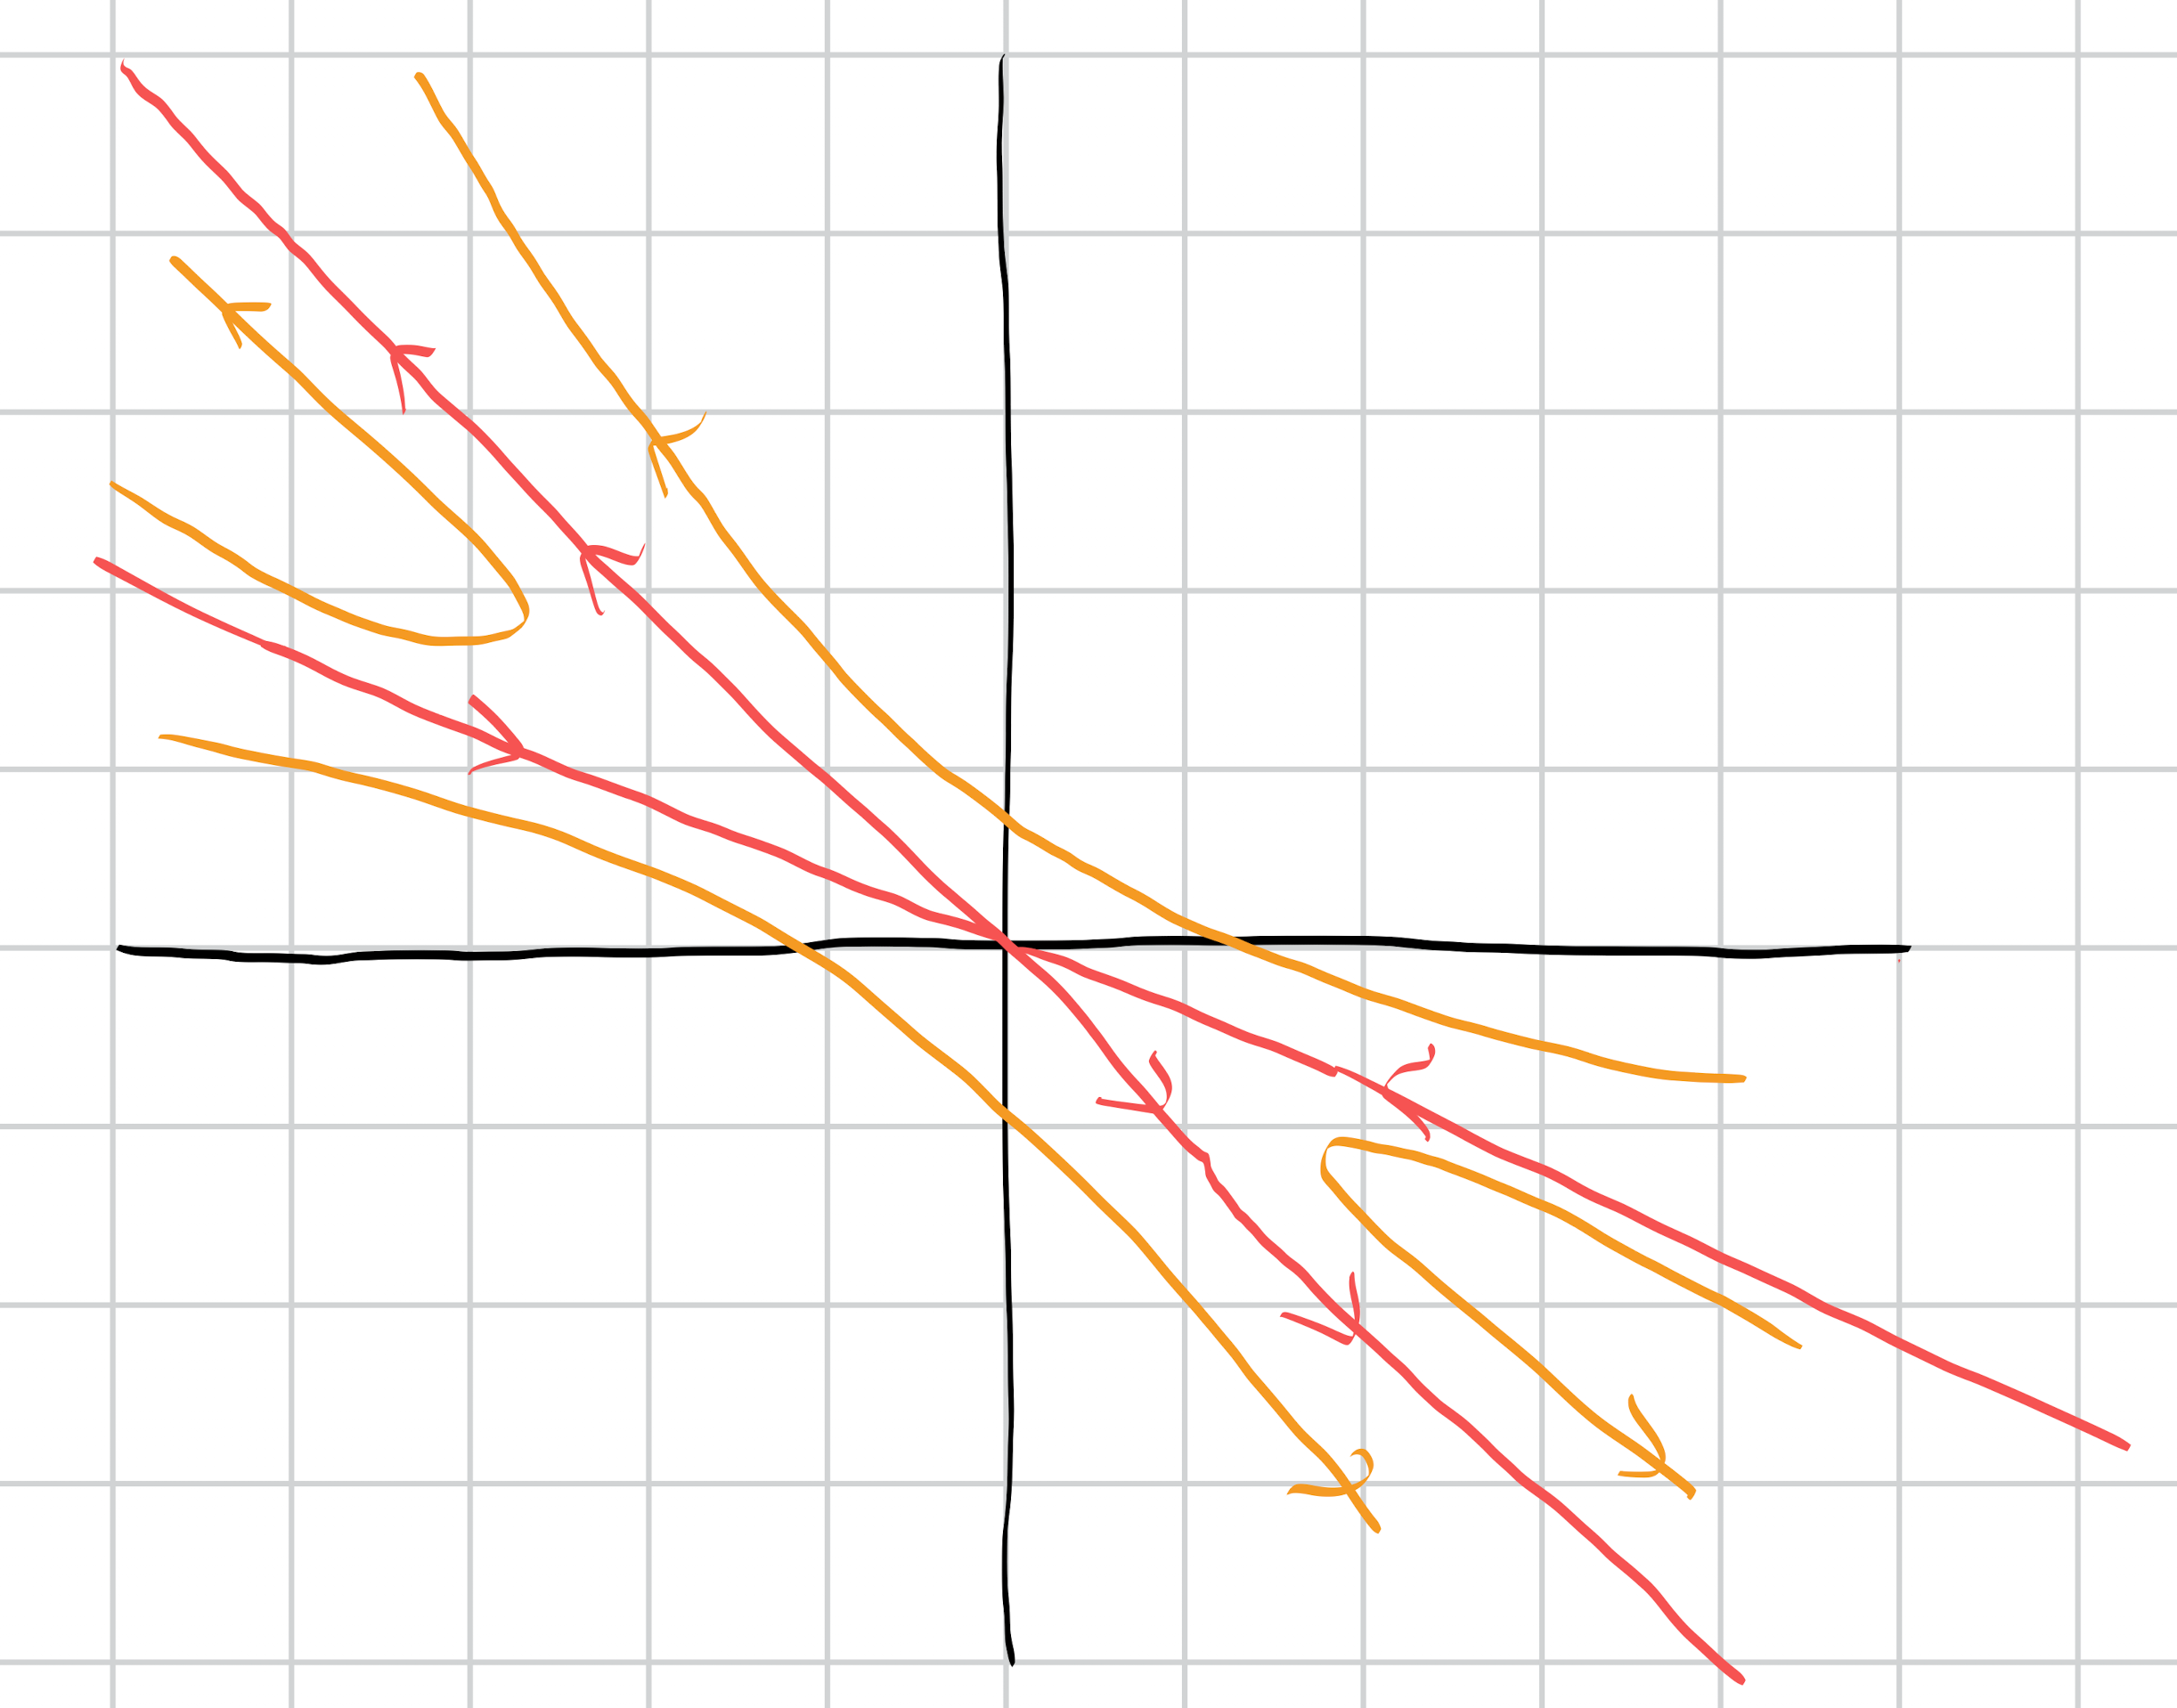
\includegraphics[width=7cm]{images/3_3_4.png}
\end{center}
\subsection{3.3, Problem 7}%
Finding the eigenvalues of the matrix, we have
\begin{align*}
  \det \begin{pmatrix}2-\lambda & 1 \\ 1 & 1 - \lambda\end{pmatrix} &= \left(\lambda - 2\right)\left(\lambda - 1\right) - 1\\
  \lambda^2 - 3\lambda + 1 &= 0,
\end{align*}
from which we get eigenvalues of $\lambda_{1,2} = \frac{3}{2}\pm \frac{\sqrt{5}}{2}$. The corresponding eigenvectors are
\begin{align*}
  \vec{v}_1 &= \begin{pmatrix}1\\ \left(-1 + \sqrt{5}\right)/2\end{pmatrix}\\
\vec{v}_2 &= \begin{pmatrix}1\\\left(-1-\sqrt{5}\right)/2\end{pmatrix}.
\end{align*}
The phase portrait is as follows.
\begin{center}
  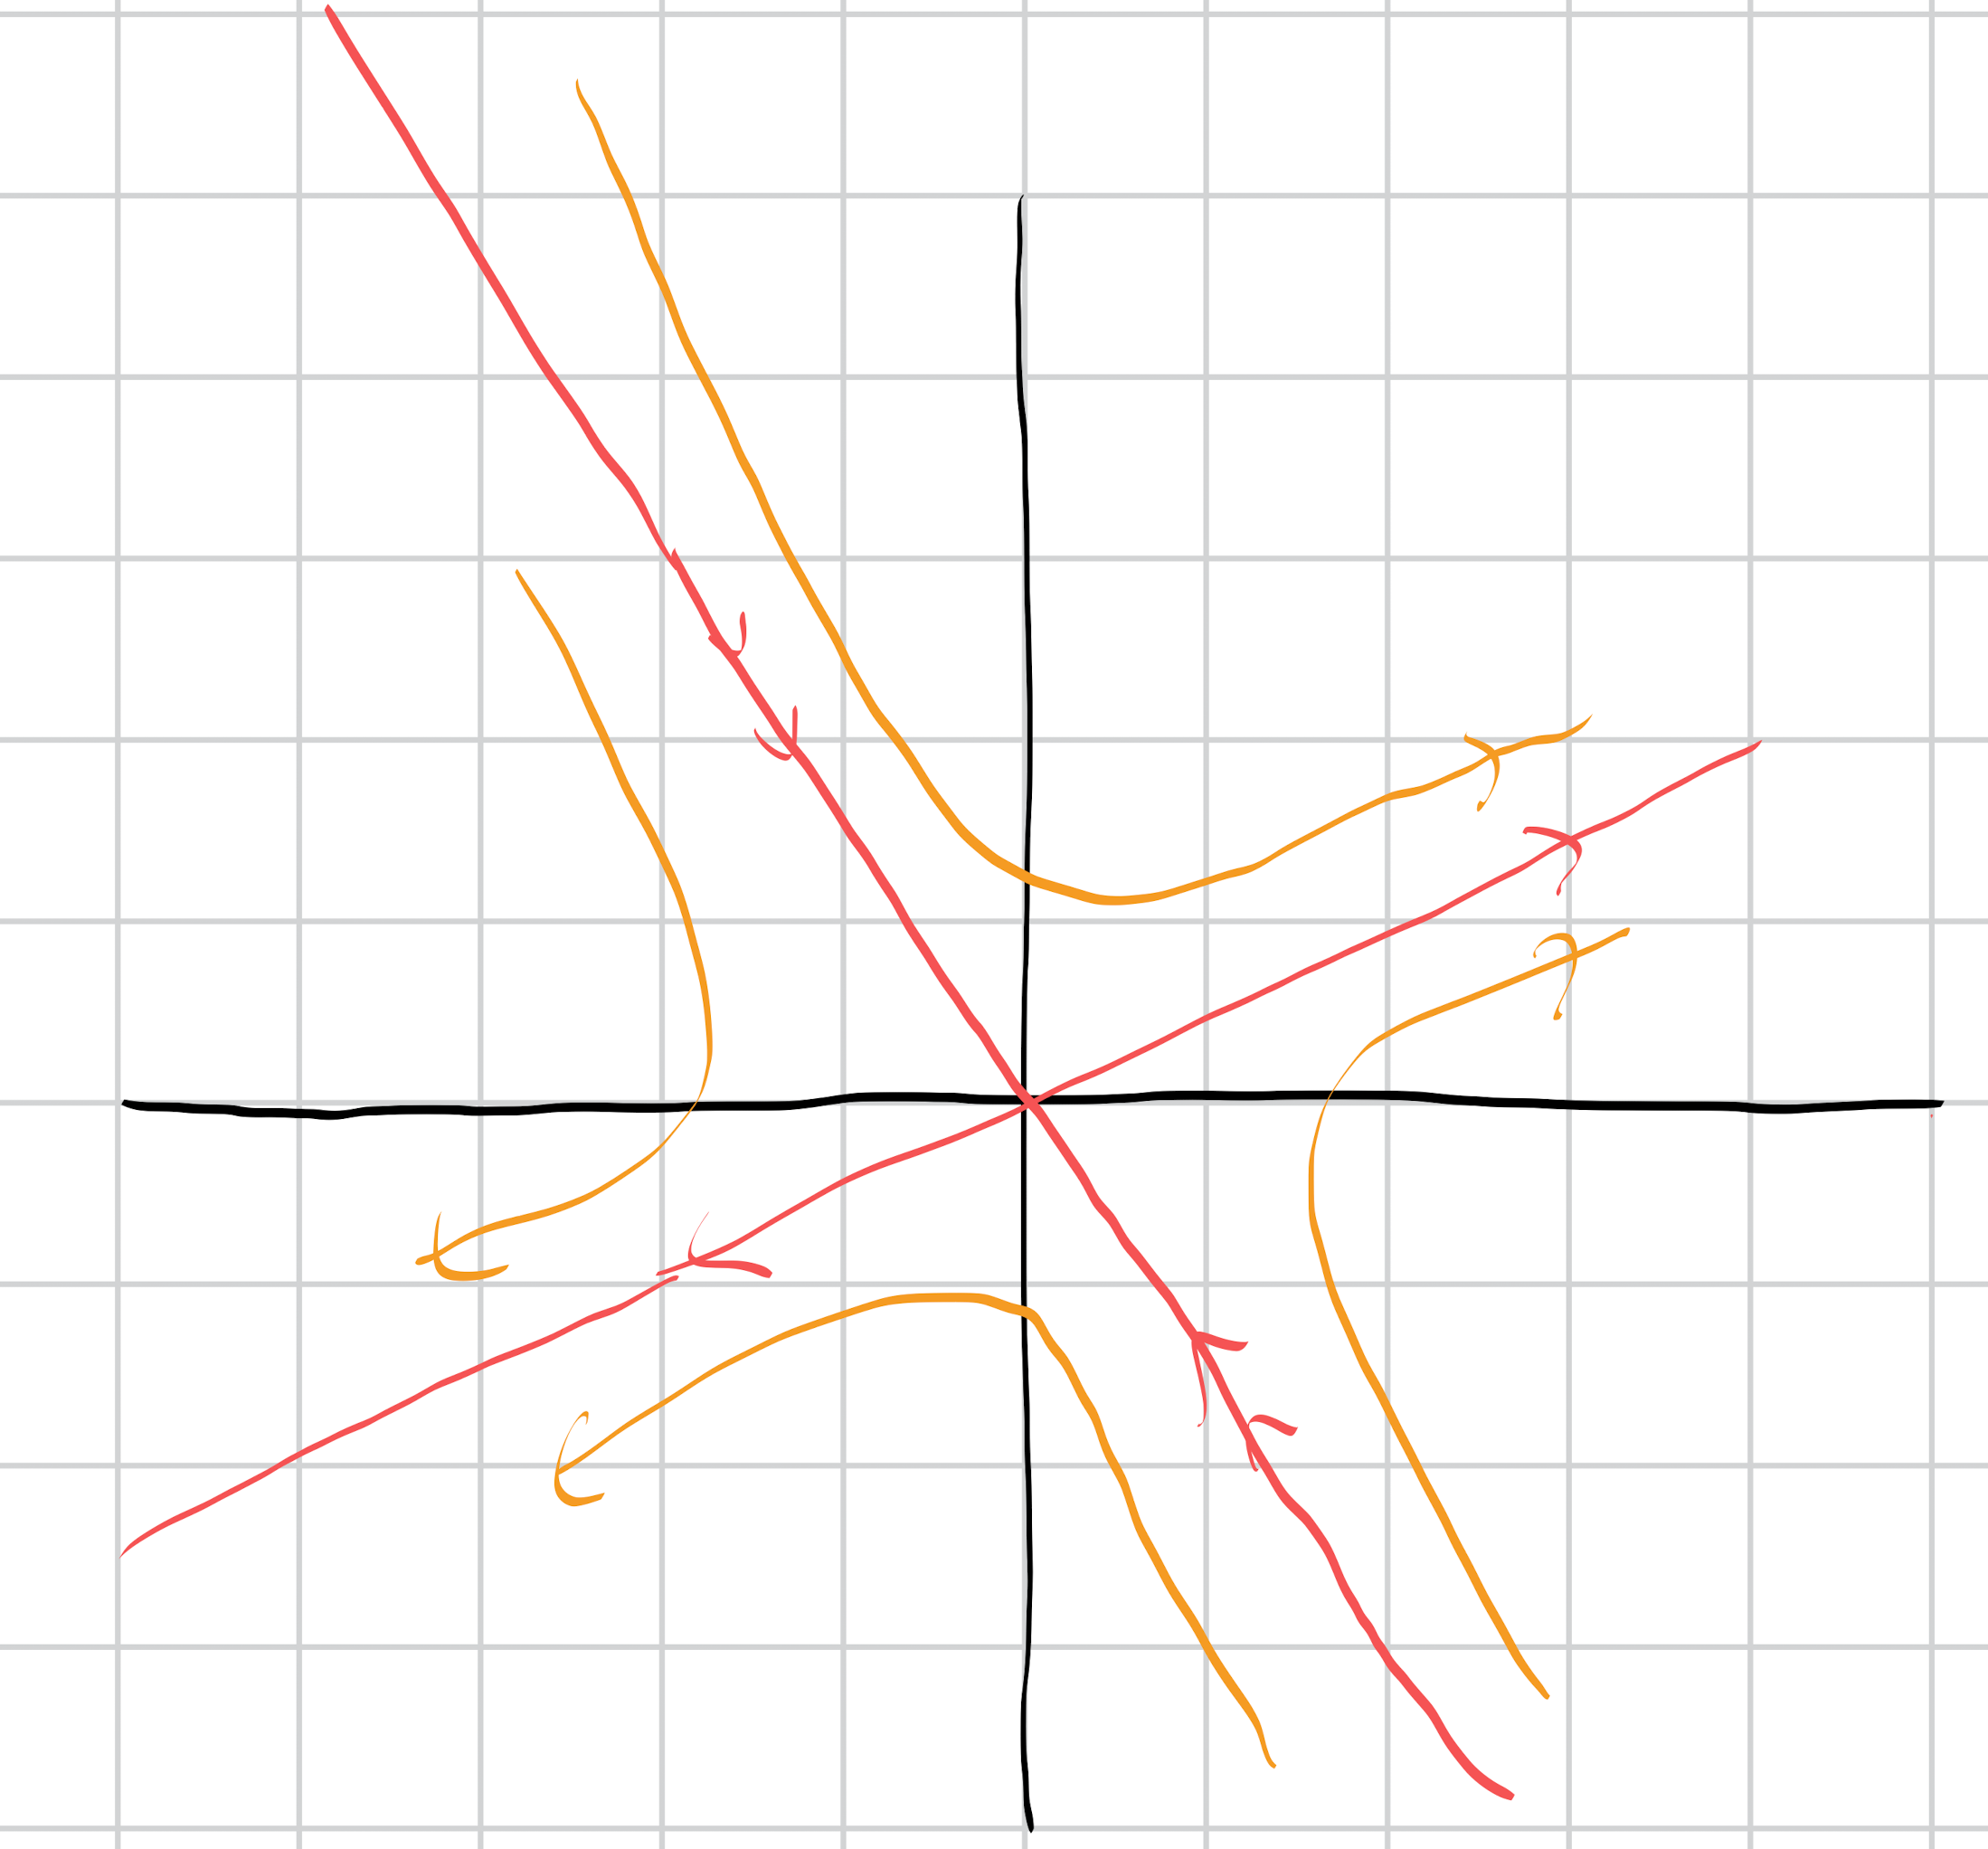
\includegraphics[width=7cm]{images/3_3_7.png}
\end{center}
\subsection{3.3, Problem 8}%
Finding the eigenvalues of the matrix, we have
\begin{align*}
  \det \begin{pmatrix}-1-\lambda & -2 \\ 1 & -4-\lambda\end{pmatrix} &= \left(\lambda + 4\right)\left(\lambda + 1\right) + 2\\
  \lambda^2 + 5\lambda + 6 &= 0\\
  \left(\lambda + 3\right)\left(\lambda + 2\right) &= 0,
\end{align*}
giving eigenvalues of $\lambda_1 = -3$ and $\lambda_2 = -2$. The corresponding eigenvectors are
\begin{align*}
  \vec{v}_1 &= \begin{pmatrix}1\\1\end{pmatrix}\\
  \vec{v}_2 &= \begin{pmatrix}2\\1\end{pmatrix}.
\end{align*}
The corresponding phase portrait is as follows.
\begin{center}
  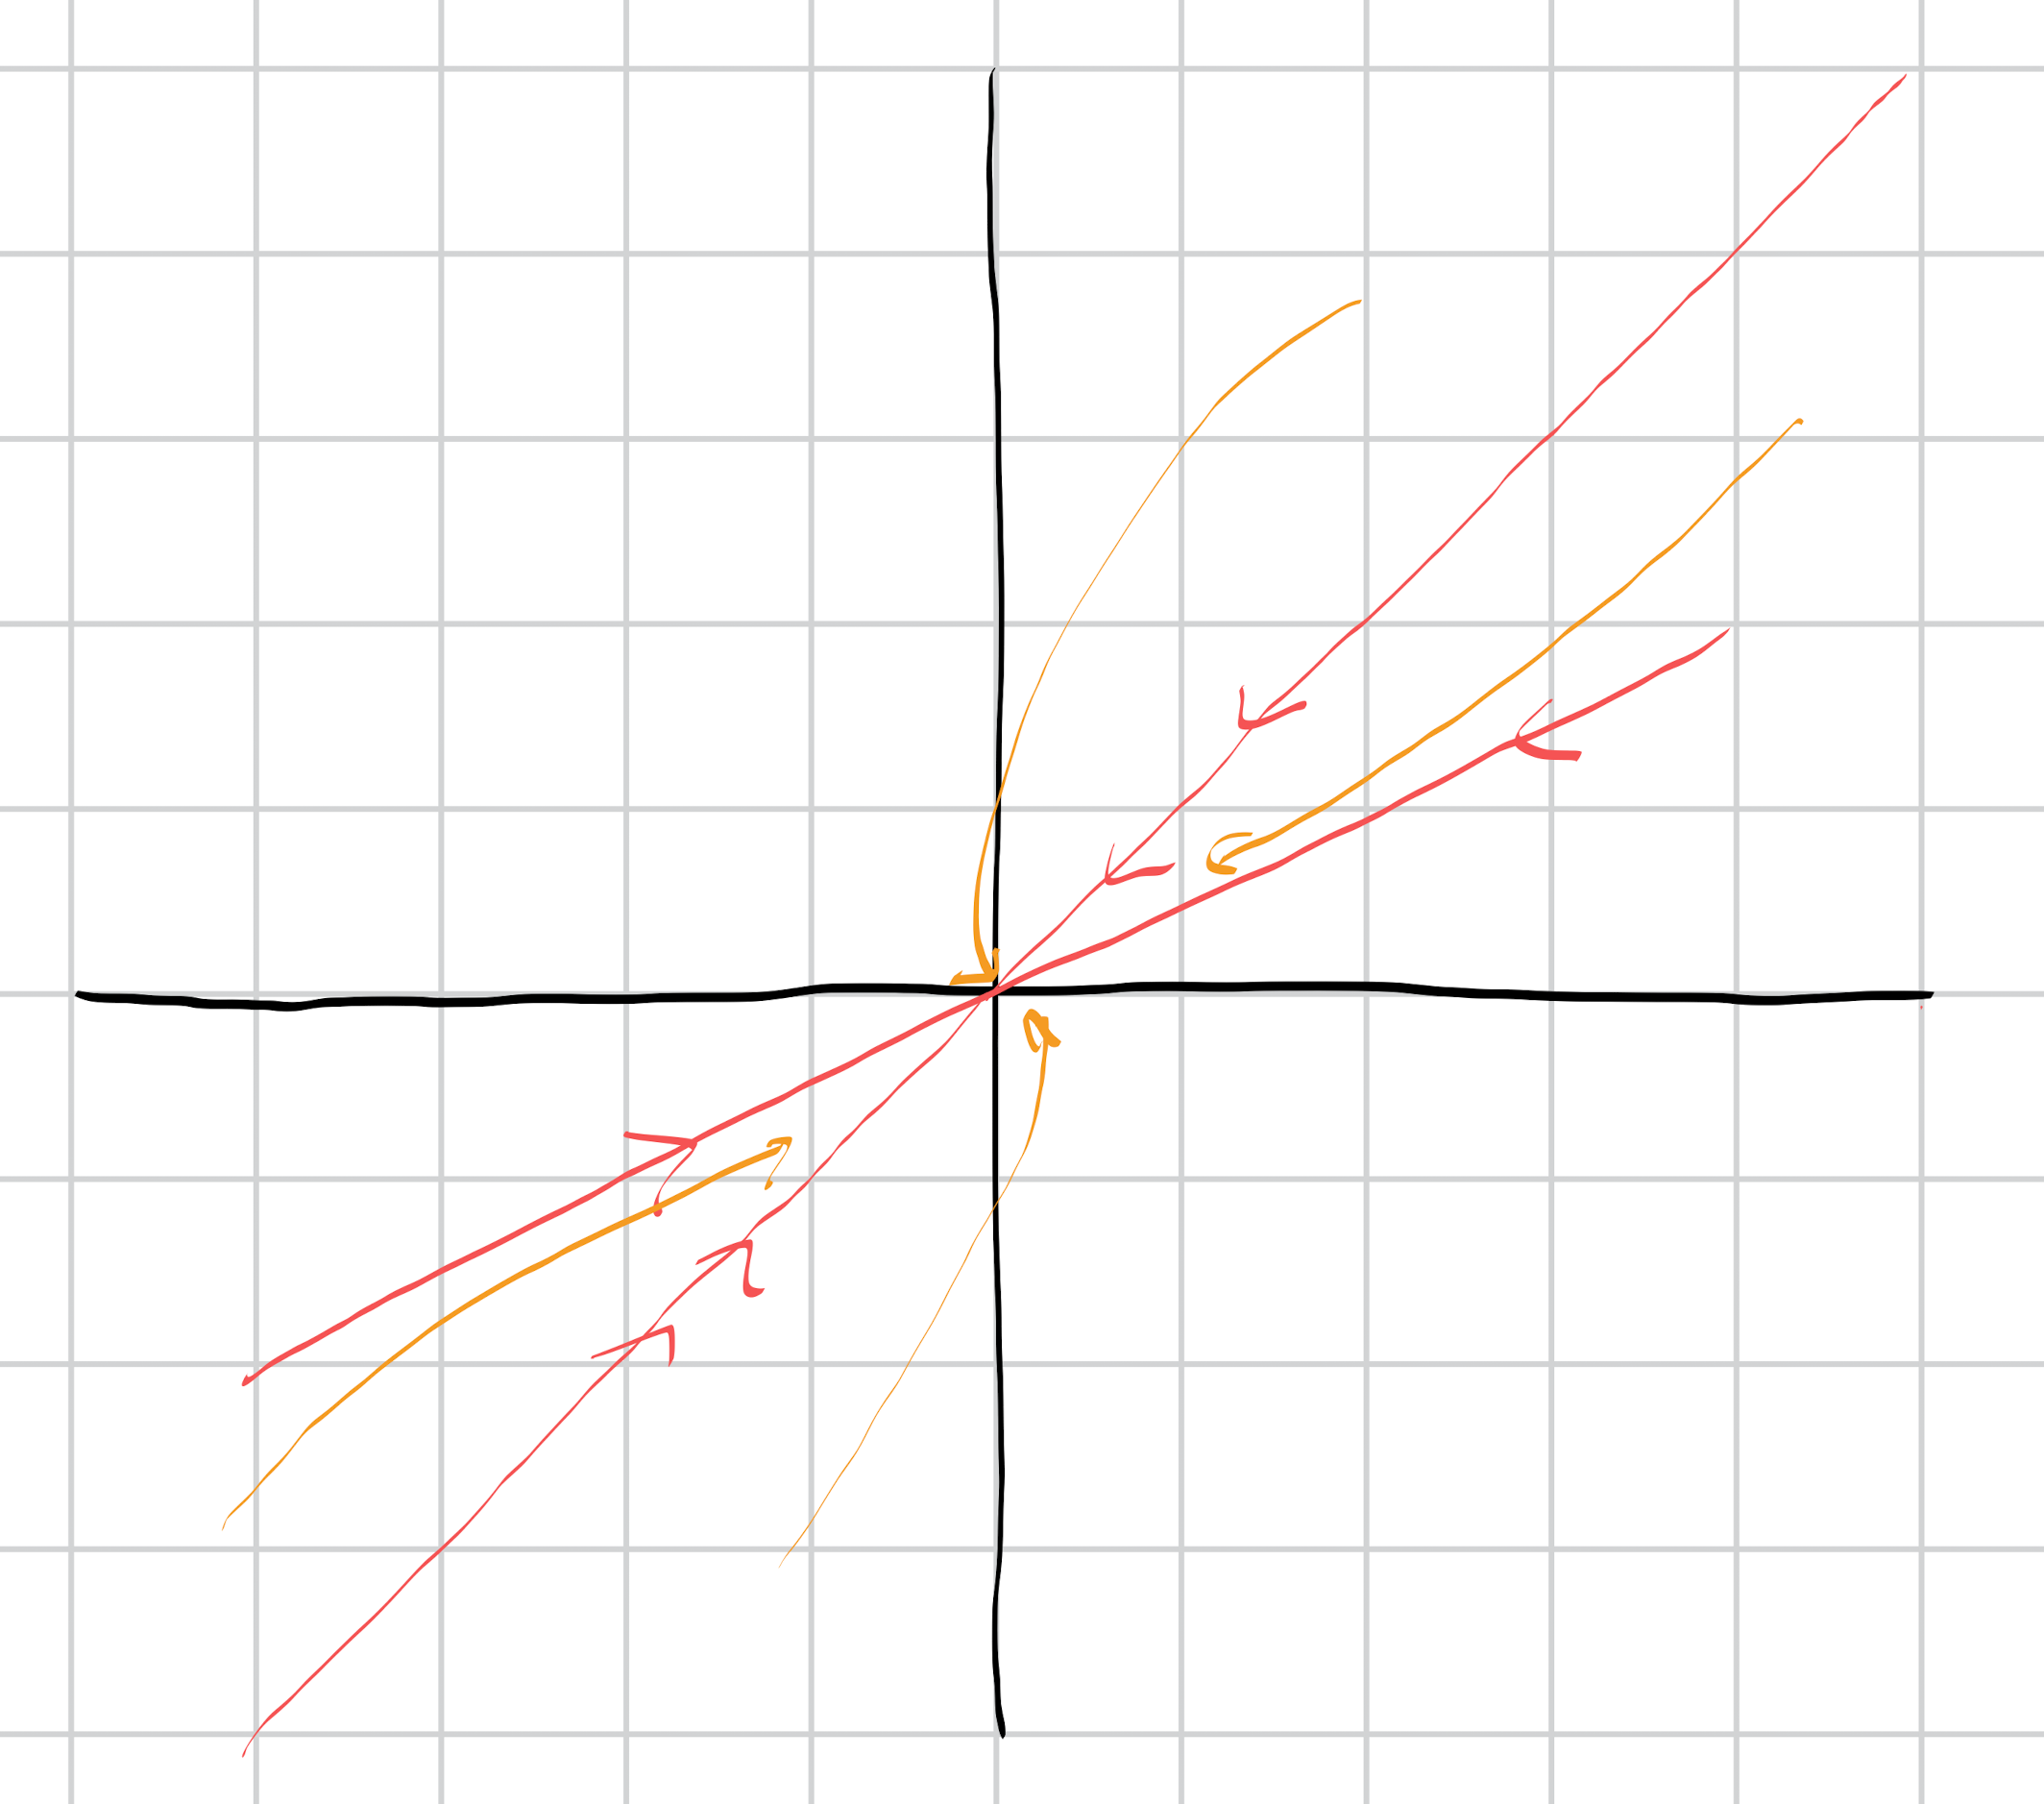
\includegraphics[width=7cm]{images/3_3_8.png}
\end{center}
\subsection{3.3, Problem 20}%
\begin{enumerate}[(a)]
  \item The equilibrium point at the origin is a saddle.
  \item The straight line solutions are 
    \begin{align*}
      \vec{Y}_1 &= e^{-4t} \begin{pmatrix}1\\-1\end{pmatrix}\\
      \vec{Y}_2 &= e^{4t} \begin{pmatrix}3\\1\end{pmatrix}
    \end{align*}
  \item I don't know how to do this problem.
\end{enumerate}
\section{Part 2}%
\subsection{3.4, Problem 1}%
\begin{align*}
  \vec{Y}_1 &= e^{t\left(1 + 3i\right)} \begin{pmatrix}2 + i \\ 1\end{pmatrix}\\
            &= e^{t}\left(\cos\left(3t\right) + i\sin\left(3t\right)\right) \left( \begin{pmatrix}2\\1\end{pmatrix} + i \begin{pmatrix}1\\0\end{pmatrix}\right)\\
            &= e^{t}\cos\left(3t\right) \begin{pmatrix}2\\1\end{pmatrix} - e^{t}\sin\left(3t\right) \begin{pmatrix}1\\0\end{pmatrix} + ie^{t}\left(\cos\left(3t\right) \begin{pmatrix}2\\1\end{pmatrix} + \sin\left(3t\right) \begin{pmatrix}1\\0\end{pmatrix}\right).
\end{align*}
Thus, the general solution is
\begin{align*}
  \vec{Y}(t) &= k_1e^{t}\cos\left(3t\right) \begin{pmatrix}2\\1\end{pmatrix} - e^{t}\sin\left(3t\right) \begin{pmatrix}1\\0\end{pmatrix} + k_2e^{t}\left(\cos\left(3t\right) \begin{pmatrix}2\\1\end{pmatrix} + \sin\left(3t\right) \begin{pmatrix}1\\0\end{pmatrix}\right).
\end{align*}
\subsection{3.4, Problem 2}%
\begin{align*}
  \vec{Y}_2 &= e^{t\left(-2 + 5i\right)} \begin{pmatrix}1\\4-3i\end{pmatrix}\\
            &= e^{-2t}\left(\cos\left(5t\right) \begin{pmatrix}1\\4\end{pmatrix} + 3\sin\left(5t\right) \begin{pmatrix}0\\1\end{pmatrix}\right) + ie^{-2t} \left( -3\cos\left(2t\right)\begin{pmatrix}0\\1\end{pmatrix} + \sin\left(5t\right) \begin{pmatrix}1\\4\end{pmatrix}\right).
\end{align*}
Thus, the general solution is
\begin{align*}
  \vec{Y}(t) &= k_1e^{-2t}\left(\cos\left(5t\right) \begin{pmatrix}1\\4\end{pmatrix} + 3\sin\left(5t\right) \begin{pmatrix}0\\1\end{pmatrix}\right) + k_2e^{-2t} \left( -3\cos\left(2t\right)\begin{pmatrix}0\\1\end{pmatrix} + \sin\left(5t\right) \begin{pmatrix}1\\4\end{pmatrix}\right).
\end{align*}
\subsection{3.4, Problem 9 (a)}%
The eigenvalues are at $\pm 2i$. The corresponding eigenvectors are
\begin{align*}
  \vec{v}_1 &= \begin{pmatrix}-i\\1\end{pmatrix}.
\end{align*}
Thus, we get
\begin{align*}
  \vec{Y}_1(t) &= e^{2it} \begin{pmatrix}-i\\1\end{pmatrix}\\
               &= \left(\cos\left(2t\right) + i\sin\left(2t\right)\right) \left( \begin{pmatrix}0\\1\end{pmatrix} - i \begin{pmatrix}1\\0\end{pmatrix}\right)\\
               &= \cos\left(2t\right) \begin{pmatrix}0\\1\end{pmatrix} + \sin\left(2t\right) \begin{pmatrix}1\\0\end{pmatrix} + i\left(-\cos\left(2t\right) \begin{pmatrix}0\\1\end{pmatrix} + \sin\left(2t\right) \begin{pmatrix}1\\0\end{pmatrix}\right).
\end{align*}
The general solution is, thus
\begin{align*}
  \vec{Y}(t) &= k_1\left(\cos\left(2t\right) \begin{pmatrix}0\\1\end{pmatrix} + \sin\left(2t\right) \begin{pmatrix}1\\0\end{pmatrix}\right) + k_2\left(-\cos\left(2t\right) \begin{pmatrix}0\\1\end{pmatrix} + \sin\left(2t\right) \begin{pmatrix}1\\0\end{pmatrix}\right).
\end{align*}
\end{document}
